\documentclass{beamer}
\beamertemplatenavigationsymbolsempty % remove the default navigation symbols
% default colors
% used in standalone pictures and when no university is selected
\definecolor{black}{HTML}{000000}
\definecolor{green}{HTML}{33BB33}
\definecolor{red}{HTML}{BB3333}
\definecolor{orange}{HTML}{BB6600}
\definecolor{blue}{HTML}{3333BB}
\definecolor{uulmaccent}{HTML}{999999}

\definecolor{uulmlogoblue}{named}{blue}
\definecolor{uulmblue}{named}{blue}

\ifdarkmode
	\colorlet{green}{green!85!white}
	\colorlet{red}{red!85!white}
	\colorlet{orange}{orange!85!white}
	\colorlet{blue}{blue!85!white}
	\setbeamercolor{section in toc shaded}{fg=black}
	\setbeamertemplate{section in toc shaded}[default][50]
\fi


\setbeamersize{text margin left=0mm,text margin right=0mm}

\usepackage{tikz}
\usepackage{pgfplots}
\pgfplotsset{
	width=\linewidth,
	height=.75\linewidth,
	xlabel near ticks,
	ylabel near ticks,
	/pgf/number format/.cd,use comma,1000 sep={.},
}

\begin{document}

	% Effectivity of Interaction Testing \mysource{\href{https://ieeexplore.ieee.org/document/1321063}{Kuhn et al.\ 2004}}
	\begin{frame}[plain]
		\centering\Large
		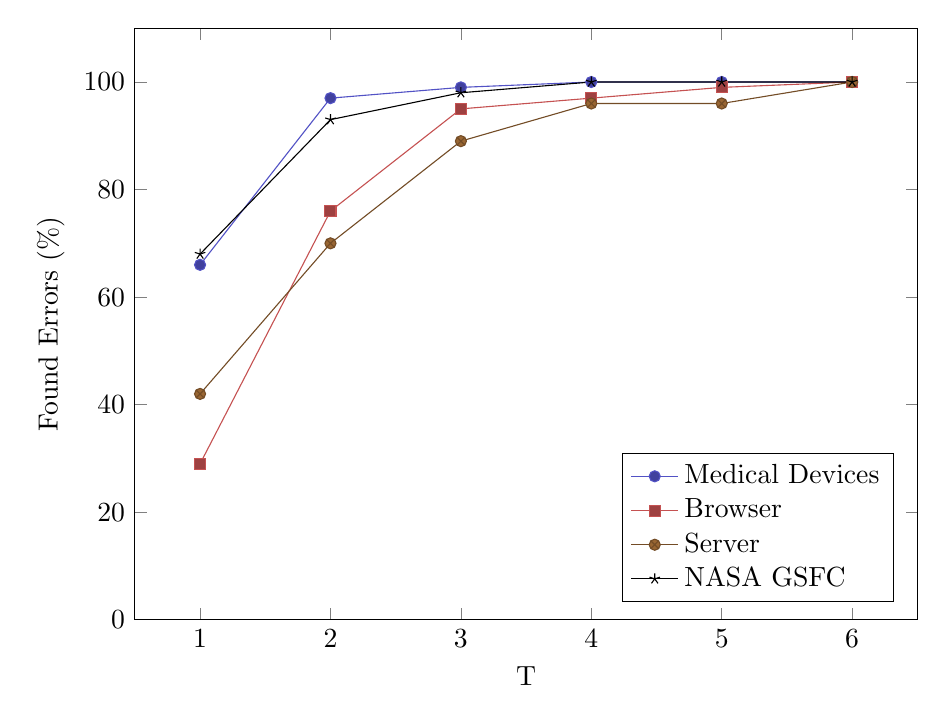
\begin{tikzpicture}
			\begin{axis}[
				width=.95\linewidth,
				ymin=0,ymax=110,
				xlabel=T,
				ylabel=Found Errors (\%),
				xtick={1,2,3,4,5,6},
				legend style={at={(0.97,0.03)},anchor=south east},
				legend cell align=left,
				]
				\addplot coordinates {(1,66) (2,97) (3,99) (4,100) (5,100) (6,100)};
				\addplot coordinates {(1,29) (2,76) (3,95) (4,97) (5,99) (6,100)};
				\addplot coordinates {(1,42) (2,70) (3,89) (4,96) (5,96) (6,100)};
				\addplot coordinates {(1,68) (2,93) (3,98) (4,100) (5,100) (6,100)};
				\legend{Medical Devices,Browser,Server,NASA GSFC}
			\end{axis}
		\end{tikzpicture}
	\end{frame}

	% Time in Minutes to Compute Sample
	\begin{frame}[plain]
		\centering
		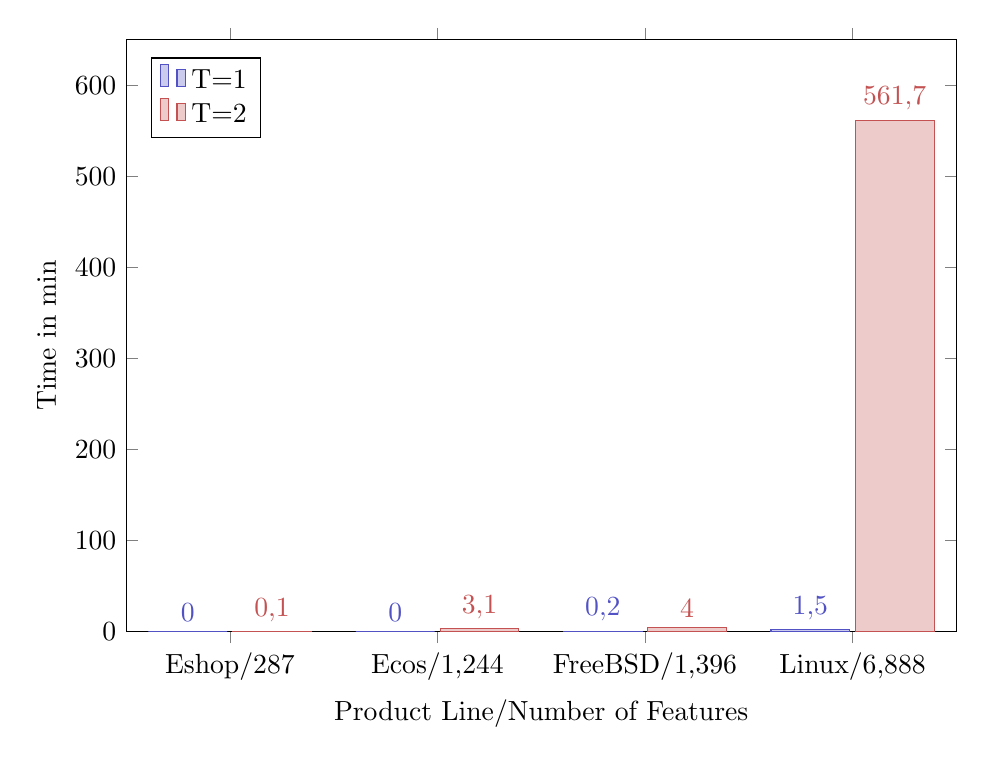
\begin{tikzpicture}
			\begin{axis}[
				ybar,
				bar width=10mm,
				ymin=0,ymax=650,
				xmin=-.5,xmax=3.5,
				xlabel=Product Line/Number of Features,
				ylabel=Time in min,
				xtick={0,1,2,3},
				xticklabels={Eshop/287,{Ecos/1,244},{FreeBSD/1,396},{Linux/6,888}},
				nodes near coords={\pgfmathprintnumber[precision=1,fixed]{\pgfplotspointmeta}},
				legend style={at={(0.03,0.97)},anchor=north west},
				legend cell align=left,
				]
				\addplot coordinates {(0,0) (1,0) (2,.2) (3,1.5)};
				\addplot coordinates {(0,.1) (1,3.1) (2,4.0) (3,561.7)};
				%	\addplot coordinates {(0,7.6) };
				\legend{T=1,T=2,T=3}
			\end{axis}
		\end{tikzpicture}
	\end{frame}

	% Number of Configurations in Sample
	\begin{frame}[plain]
		\centering
		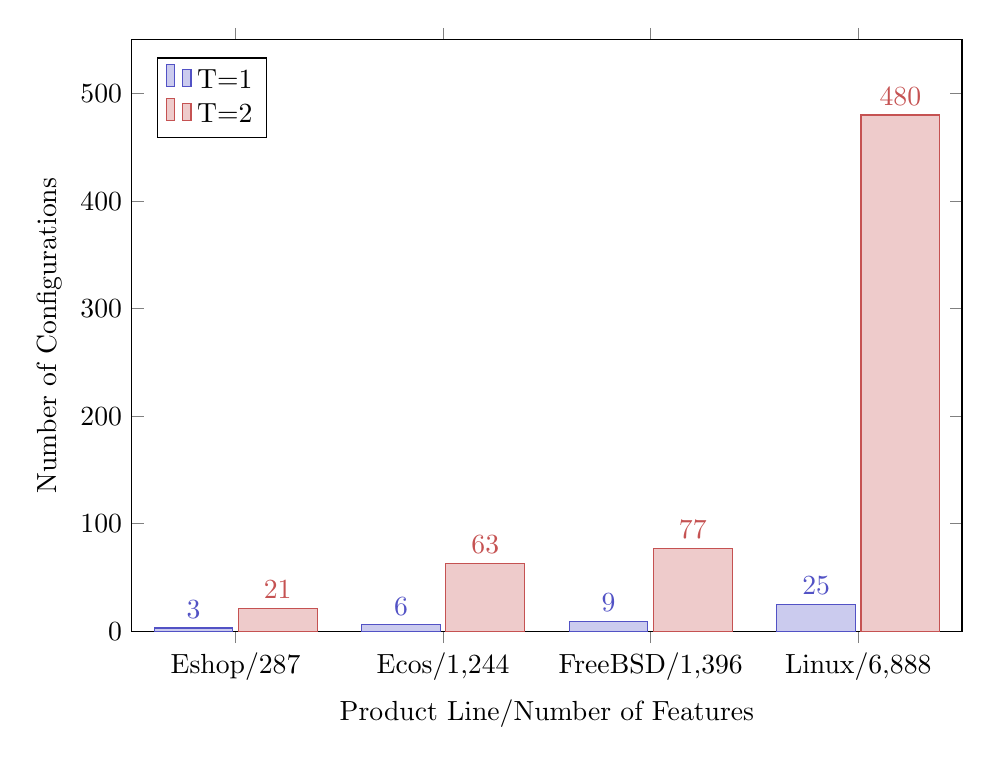
\begin{tikzpicture}
			\begin{axis}[
				ybar,
				bar width=10mm,
				ymin=0,ymax=550,
				xmin=-.5,xmax=3.5,
				xlabel=Product Line/Number of Features,
				ylabel=Number of Configurations,
				xtick={0,1,2,3},
				xticklabels={Eshop/287,{Ecos/1,244},{FreeBSD/1,396},{Linux/6,888}},
				nodes near coords={\pgfmathprintnumber[precision=0]{\pgfplotspointmeta}},
				legend style={at={(0.03,0.97)},anchor=north west},
				legend cell align=left,
				]
				\addplot coordinates {(0,3) (1,6) (2,9) (3,25)};
				\addplot coordinates {(0,21) (1,63) (2,77) (3,480)};
				%	\addplot coordinates {(0,108) };
				\legend{T=1,T=2,T=3}
			\end{axis}
		\end{tikzpicture}
	\end{frame}

	% Number of Configurations in Pairwise Sample
	\begin{frame}[plain]
		\centering
		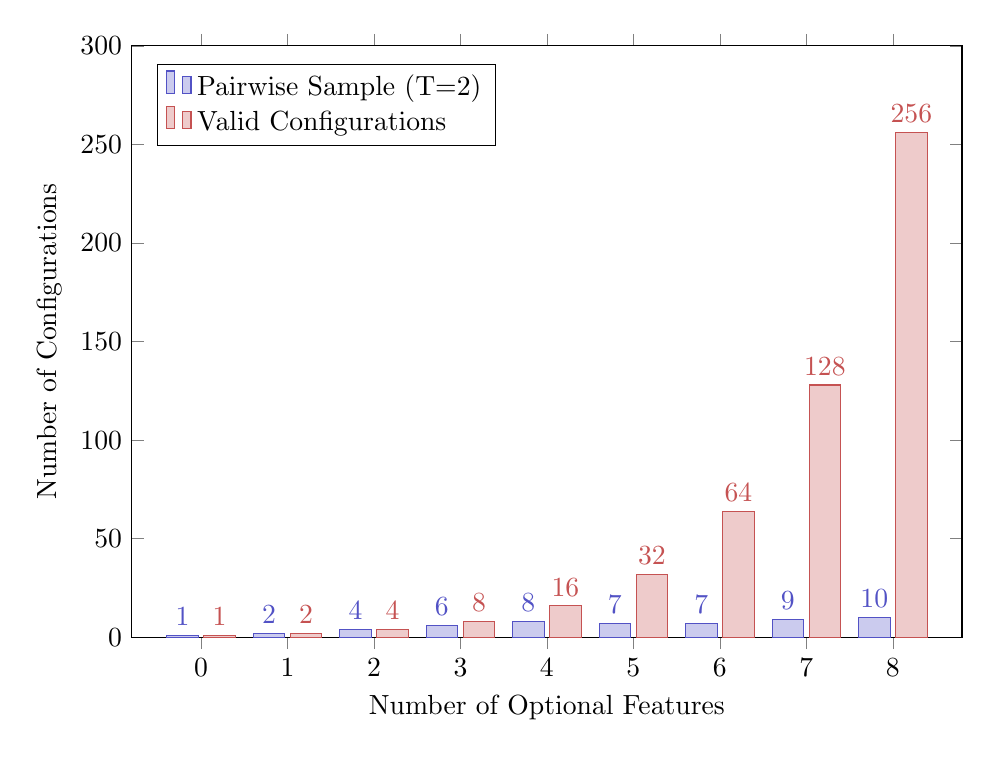
\begin{tikzpicture}
			\begin{axis}[
				ybar,
				bar width=4mm,
				ymin=0,ymax=300,
				xlabel=Number of Optional Features,
				ylabel=Number of Configurations,
				nodes near coords={\pgfmathprintnumber[precision=0]{\pgfplotspointmeta}},
				legend style={at={(0.03,0.97)},anchor=north west},
				legend cell align=left,
				]
				\addplot coordinates {(0,1) (1,2) (2,4) (3,6) (4,8) (5,7) (6,7) (7,9) (8,10)};
				\addplot coordinates {(0,1) (1,2) (2,4) (3,8) (4,16) (5,32) (6,64) (7,128) (8,256)};
				\legend{Pairwise Sample (T=2),Valid Configurations}
			\end{axis}
		\end{tikzpicture}
	\end{frame}

	% Number of Configurations in T-Wise Sample
	\begin{frame}[plain]
		\centering
		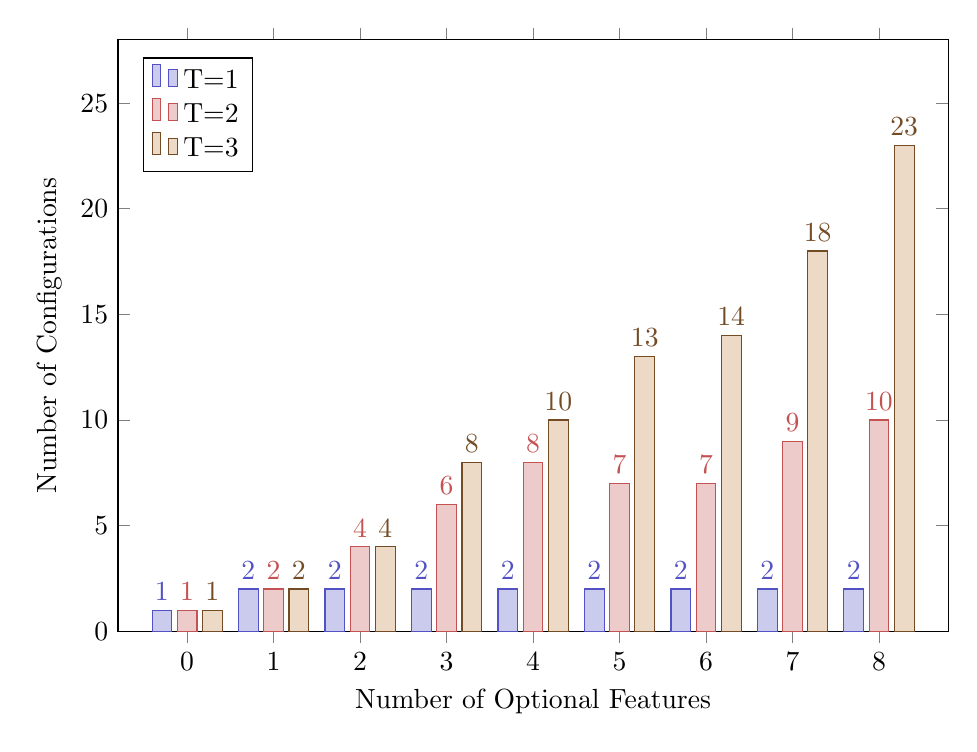
\begin{tikzpicture}
			\begin{axis}[
				ybar,
				bar width=2.5mm,
				ymin=0,ymax=28,
				xlabel=Number of Optional Features,
				ylabel=Number of Configurations,
				nodes near coords={\pgfmathprintnumber[precision=0]{\pgfplotspointmeta}},
				legend style={at={(0.03,0.97)},anchor=north west},
				legend cell align=left,
				]
				\addplot coordinates {(0,1) (1,2) (2,2) (3,2) (4,2) (5,2) (6,2) (7,2) (8,2)};
				\addplot coordinates {(0,1) (1,2) (2,4) (3,6) (4,8) (5,7) (6,7) (7,9) (8,10)};
				\addplot coordinates {(0,1) (1,2) (2,4) (3,8) (4,10) (5,13) (6,14) (7,18) (8,23)};
				\legend{T=1,T=2,T=3}
			\end{axis}
		\end{tikzpicture}
	\end{frame}

\end{document}
